%%%%%%%%%%%%%%%%%%%%%%%%%%%%%%%%%%%%%%%%%%%%%%%%%%%%%%%%%%%%%%%%%%%%%%%%%%%%%%%%
%science.tex: Chapter on DM physics:
%%%%%%%%%%%%%%%%%%%%%%%%%%%%%%%%%%%%%%%%%%%%%%%%%%%%%%%%%%%%%%%%%%%%%%%%%%%%%%%%
\chapter{Dark Matter}
\label{chapter:dm}
%%%%%%%%%%%%%%%%%%%%%%%%%%%%%%%%%%%%%%%%%%%%%%%%%%%%%%%%%%%%%%%%%%%%%%%%%%%%%%%%

New phenomena have puzzled physicists throughout history, but the confusion surrounding dark matter
-- estimated to be roughly 85\% of the total matter in the universe -- is surely one of the biggest
puzzles. While many astronomical observations at various scales have confirmed the existence of
dark matter, we have not yet seen any observations of its particle interacting with our detectors.
This has ruled out many models for dark matter's particle nature, but there are still many more
available which can both explain the current observations of dark matter gravitational and
cosmological effects while skirting the limitations defined by the \emph{lack} of observation in
particle experiments.

\section{Dark Matter?}
The term \ac{dm} rose out of a brutally honest description of the present level of understanding.
``Matter'' originates from comparison to the particles that make ourselves up and with which we are
familiar -- both this new phenomena and our normal ``stuff'' interact gravitationally, attracting
other groups of ``matter'' into complex cosmological systems. The adjective ``dark'' refers to the
literal fact that we cannot see it with our telescopes. Other matter out in the universe can be
seen via the light that it gives off (or reflects), so the fact that this matter \emph{is not}
visible in this way motivates the adjective.

That is it. \acf{dm} is merely a shorthand for this aspect of the universe that is both known to
exist within the cosmos and whose particle nature is completely unknown.

\section{Evidence for Dark Matter}
\label{sec:dm:evidence}

The first (replicable) evidence physicists had for an unseen material floating throughout the
universe was the observation of galactic rotation curves
\cite{rubin-rotationcurve-1980,rotationcurve-2000}. These observations measure the speed of
different stars within a galaxy and compare this speed to the distance of that star from the center
of the galaxy. We can calculate this relationship using \ac{gr}
\cite{rotationcurve-predictions-2007} and the observations differ drastically from this
calculation. The stars within galaxies we've observed move much faster than \ac{gr} would predict
(\cref{fig:rotation-curve}) leaving us with two explanations: either \ac{gr} is not the correct
theory to use in this situation or there is more un-seen mass floating within the galaxy allowing
these stars to move faster without leaving the galactic orbit.

Other indirect measurements give us additional ways to access information about this odd phenomena.
Within the framework of \ac{gr}, since energy and mass actually warp the fabric of spacetime, we
expect to see light itself follow a bent path around massive objects - a phenomenum that is called
gravitational lensing and is observed and well modeled by \ac{gr}'s predictions
\cite{gravlensing-2004}. The accuracy of \ac{gr} within this context -- a mass and distance scale
similar to the rotation curve oddities also observed -- put more requirements on any modified
theory of gravity that could both explain the rotation curves and gravitational lensing.
Additionally, measurements on some of the largest scales and from the early universe display signs
of a certain mass density attributed matter that does not interact in the same ways as our normal
matter (called ``baryonic'' matter).

In the early universe, standard matter was compressed into high densities and existed at high
temperature creating a sea of plasma. Gravity attracts while pressure from the squeezing of this
plasma repulses which produces oscillations in the density of matter in space and time. The
repulsive pressure within the plasma originates from particles interacting electromagnetically with
each other, so the oscillations would be disrupted by the presence of extra matter interacting
gravitationally but not interacting electromagnetically. These \ac{bao} are imprinted on our
snapshot of this early-universe plasma, the \ac{cmb}, which we can measure with a high degree of
accuracy and fit to various models of what existed at this time of the universe. The best fit of
these models corresponds to only $\sim 5\%$ of the mass density being normal matter like we see
today (``baryonic'') while the rest is composed of material that only significantly interacts
gravitationally \cite{planck-cmb-2015}.

Additional astromomy observations from Type1a supernovae \cite{type1a-supernova-2010}, fitting
models of big bang nucleosynthesis \cite{nucleosynthesis-1998}, and constraints on non-particulate
theories explaining these phenomena (for example mini black holes
\cite{constraints-primordial-black-holes-2021}) all allow us to conclude pretty comfortably that
\ac{dm} exists as a particle in our universe.

\begin{figure}
  \centering
  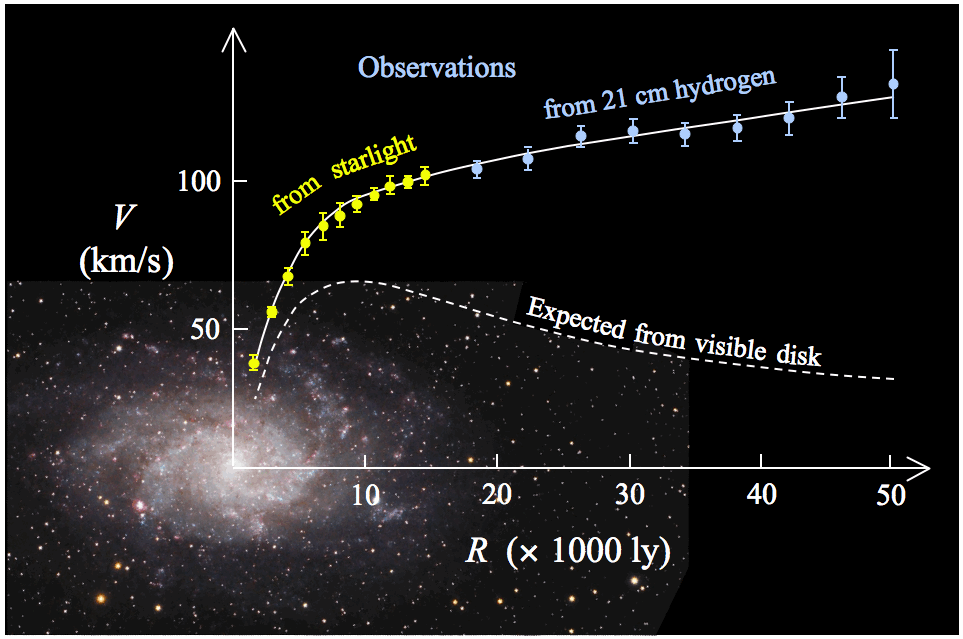
\includegraphics[width=0.6\textwidth]{figures/theory/rotation-curve-evidence-for-dm.png}
  \caption{
    Depiction of the velocity of stars within a galaxy as a function of their distance
    from the galactic center. The dotted line is a prediction of this relationship using
    \ac{gr} along with the mass tabulated from the visible starts while the data points
    (and the solid line fitted to them) are what are actually seen in galaxies today.
  }
  \label{fig:rotation-curve}
\end{figure}

\section{Particle Nature of Dark Matter}
The theoretical possibilities explaining \ac{dm} are broad \cite{darksectors-2016} even when
excluding ourselves to the assumption that the \ac{dm} phenomenum is explained by the existence of
a \ac{dm} particle. The \ac{cmb} observations are tied to very early on in the existence of the
universe, so it is natural to assume that this \ac{dm} particle has existed since the start of the
universe alongside our normal matter particles. With this in mind, we can outline a few criteria
that must be met by a proposed \ac{dm} candidate.
\begin{itemize}
  \item \textbf{Dark} There has been no detection of these particles via the light observed with our telescopes;
        therefore, the \ac{dm} has to not interact via the electromagnetic force.
  \item \textbf{Long Living} Measurements of \ac{dm}'s mass density and presence agree across time
        (from as early as the \ac{cmb} era), so \ac{dm} needs to have a long lifetime.
  \item \textbf{Universal Density} Since we can indirectly measure a \ac{dm} mass density on
        cosmological scales, we impose the requirement that any \ac{dm} model needs to allow for
        this density.
  \item \textbf{Thermal Relic} Both \ac{dm} and standard matter have similar
        cosmological densities, so we expect some interaction (even a weak one) should connect their
        origins to the early universe allowing both to exist from the Big Bang. This criterion is
        not as firm as the others (\ac{dm} models correctly describing the current observations while
        avoiding this criterion do exist); nevertheless, this criterion is well motivated and it is
        satisfied by all of the models for \ac{dm} studied in this work.
\end{itemize}
Even with these assumptions and the requirements they imply, there still exist a plethora of
theoretical models that can satisfy all of them.

The upside is that a thermal-relic assumption closely connects the mass of individual \ac{dm}
particles to the interaction strength it has with standard matter. In this assumption, the \ac{dm}
evolves along with the universe allowing its number density to follow the density of standard
matter until the standard matter does not have enough energy to produce more \ac{dm}. While the
universe continues to expand, the \ac{dm} continues to decay into standard matter until it becomes
too sparse to annihilate with itself and is thus ``frozen'' at a specific number density. Since
this ``frozen'' density changes depending on how easy it is for the \ac{dm} to interact with
standard matter, the ``frozen'' number density goes down as the interaction strength increases
(\cref{fig:number-density}). The additional requirement of the observed astronomical \emph{mass}
density connects the mass of individual \ac{dm} particles to their interaction strength with
standard matter.
\begin{equation}\label{eqn:dm-mass-interaction-strength-connection}
  m_\chi \leftrightarrow \text{observed mass density}
  \leftrightarrow \frac{dN}{dV} \leftrightarrow
  \text{thermal relic hypothesis} \leftrightarrow
  \langle\sigma v\rangle
\end{equation}
This connection allows us to define strict ``thermal relic targets'' which can help be measuring
sticks for how well our experiments search for \ac{dm} (these targets will appear in plots later).

\begin{figure}
  \centering
  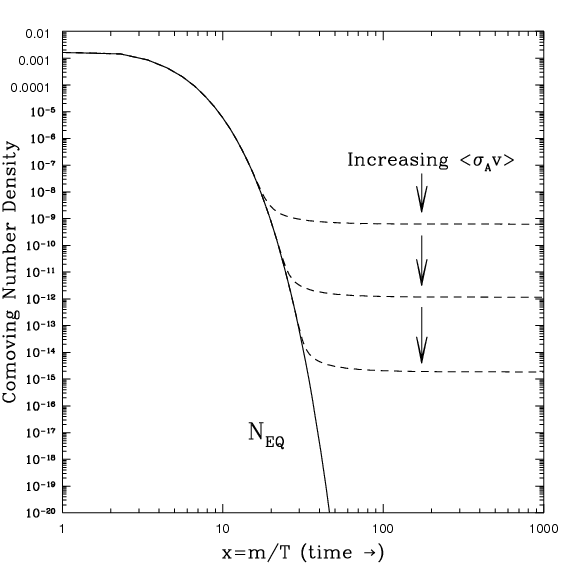
\includegraphics[width=0.5\textwidth]{figures/theory/number-density-at-freeze-out.png}
  \caption{
    From \cite{thermal-freezeout-diagram-1996}, the co-moving cosmological number density of \ac{dm} as a function of the universe
    temperature. As the universe cools, the number density decreases until the \ac{dm}
    becomes too sparse to interact with other \ac{dm} particles, ``freezing'' to a specific
    number density until today.
  }
  \label{fig:number-density}
\end{figure}

In addition to the connection between interaction strength and particle mass implied by the thermal
relic hypothesis, it also puts some loose bounds on mass of individual particles
(\cref{fig:dm-mass-scale}). If the mass is too low (approximately below the mass of the electron
$m_e$), then it is not feasible within our early-universe models to produce enough \ac{dm} to match
the observed \ac{dm} density currently frozen in. Similarly, if the mass is too high ($\gtrapprox
  100~\text{TeV}$), the \ac{dm} will be too strongly coupled to the standard matter and would be
over-produced.

\begin{figure}
  \centering
  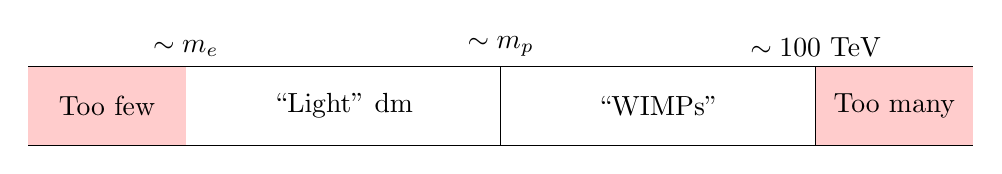
\begin{tikzpicture}
    % horizontal top/bottom lines
    \draw (0,0) -- (12,0);
    \draw (0,1) -- (12,1);
    % dividing lines along with relevant scale markers
    \draw (2,0) -- (2,1) node[above] {$\sim m_e$};
    \draw (6,0) -- (6,1) node[above] {$\sim m_p$};
    \draw (10,0) -- (10,1) node[above] {$\sim100~$TeV};
    % fill non-thermal ranges with light red
    \fill [red!20!white] (0,0) rectangle (2,1);
    \fill [red!20!white] (10,0) rectangle (12,1);
    % labels offering descriptions of ranges inside the boxes
    \node at (1,0.5) {Too few};
    \node at (4,0.5) {``Light'' \gls{dm}};
    \node at (8,0.5) {``WIMPs''};
    \node at (11,0.5) {Too many};
\end{tikzpicture}
  \caption{Mass scale of Thermal Relic \ac{dm}.
    The regions in red are excluded by applying the thermal relic assumption
    to our observations of the universe's early evolution.}
  \label{fig:dm-mass-scale}
\end{figure}

The mass scale of thermal relic \ac{dm} is further divided by the mass of the proton ($m_p$). Above
this threshold, the \ac{dm} could be interacting with standard matter through the standard Weak
Force (as described in \cref{chapter:intro}); thus, they are named \acp{wimp}. This phase space was
first searched due to its theoretical simplicitity: no new forces, just an extra particle (or two)
creating the clouds of \ac{dm} we see today. Unfortunately, these searches have not found evidence
of a \ac{wimp}-like signature\cite{supercdms-2018,damic-2020,xenon1t-2018} and the phase space has
become tighter and more exluded after many years of searching. Below $m_p$, the \ac{dm} requires a
new force which is even weaker than the Weak Force. In comparison to the heavier \acp{wimp}, this
category of \ac{dm} is called ``Light'' \ac{dm}.

\begin{figure}
  \centering
  \begin{tikzpicture}
  \begin{feynman}
    \vertex (standard) {\(\gamma\)};
    \vertex [right=of standard] (loopleft);
    \vertex [right=of loopleft] (loopright);
    \vertex [right=of loopright] (dark) {\(A'\)};

    \diagram*{
    (standard)
    -- [photon] (loopleft)
    -- [fermion, half left, edge label=\(\Phi\)] (loopright)
    -- [photon] (dark),
    (loopright)
    -- [fermion, half left, edge label=\(\Phi\)] (loopleft),
    };
  \end{feynman}
\end{tikzpicture}

  \caption{Feynman diagram of how a massive field $\Phi$ could allow for a standard photon ($\gamma$)
    to mix with a dark photon ($A'$).}
  \label{fig:photon-mixing}
\end{figure}

In general, the definition of a new force of nature is not well constrained; however, we can define
a ``baseline'' model that can represent more concrete theories in the context of our experiments.
For this situation, we postulate the existence of a massive gauge boson that represents an
additional $U_D(1)$ symmetry of nature. Since this additional symmetry has the same structure as
the electromagnetic interaction whose gauge boson is the standard photon, we generally refer to
this postulated massive boson as a dark photon. Without any additional assumptions, this new dark
photon does not interact with any standard matter, so we also assume that some previously-unknown
massive fields are able to interact with both. These other fields need to be sufficiently massive
(or sufficiently weakly coupled) so that they only allow the standard and dark photons to weakly
mix. \cref{fig:photon-mixing} diagrams how the standard and dark photons mix which can then be
effectively represented by a new vertex in our model.
\begin{equation}\label{eqn:dark-photon-ll-vertex}
  \begin{tikzpicture}
    \begin{feynman}[inline]
      \vertex (dark1) {\(A'\)};
      \vertex [right=of dark1] (loopleft);
      \vertex [right=of loopleft] (loopright);
      \vertex [right=of loopright] (gamma);
      \vertex [above right=of gamma] (ellplus1) {\(\ell^+\)};
      \vertex [below right=of gamma] (ellminus1) {\(\ell^-\)};

      \vertex [right=of gamma] (arr) {\(\Rightarrow\)};

      \vertex [right=of arr] (dark2) {\(A'\)};
      \vertex [right=of dark2, dot] (vtx) {};
      \vertex [above right=of vtx] (ellplus2) {\(\ell^+\)};
      \vertex [below right=of vtx] (ellminus2) {\(\ell^-\)};

      \diagram*{
      (dark1)
      -- [photon] (loopleft)
      -- [fermion, half left] (loopright)
      -- [photon, edge label=\(\gamma\)] (gamma),
      (loopright) -- [fermion, half left] (loopleft),
      (ellplus1) -- [fermion] (gamma) -- [fermion] (ellminus1),
      };

      \diagram*{
      (dark2) -- [photon] (vtx),
      (ellplus2) -- [fermion] (vtx) -- [fermion] (ellminus2),
      };
    \end{feynman}

    \node [right=of vtx] (eqn) {\(\propto \epsilon\)};
  \end{tikzpicture}
\end{equation}
where the mixing strength $\epsilon$ encapsulates the effect of a massive field $\Phi$ at the energies
of our experiments (presumably low enough to avoid creation of a $\Phi$ directly) and is generally
small ($\ll 1$).

This new vertex within our model for the universe enables a new process to occur: so-called ``Dark
Bremsstrahlung'' (dark brem) where a charged particle exchanges a standard photon with a nucleus
and then emits a dark photon and recoils.

\begin{figure}
  \centering
  \begin{tikzpicture}
  \begin{feynman}
    \vertex (in) {\(\ell^-\)};
    \vertex [right=of in, dot] (nuc) {};
    \vertex [below=of nuc, blob, label={below:\(Z\)}] (nucleus) {};
    \vertex [right=of nuc, dot] (emit) {};
    \vertex [above right=of emit] (recoil) {\(\ell^-\)};
    \vertex [below right=of emit] (decay) {\(A'\)};
    % \vertex [above right=of decay] (chi2) {\(\overline{\chi}\)};
    % \vertex [below right=of decay] (chi1) {\(\chi\)};

    \diagram*{
    (in) -- [fermion] (nuc) -- [fermion] (emit) -- [fermion] (recoil),
    (nucleus) -- [photon, edge label'=\(\gamma\)] (nuc),
    (emit) -- [photon] (decay),
    % (emit) -- [photon, edge label'=\(A'\)] (decay),
    % (chi2) -- [fermion] (decay) -- [fermion] (chi1),
    };
  \end{feynman}
\end{tikzpicture}

  \caption{
    Feynman diagram for the dark brem process.
  }
  \label{fig:dark-brem-feynman}
\end{figure}

But what happens to the dark photon after it interacts with standard matter via this vertex? It
cannot be the long-lived \ac{dm} we view in the universe today because this vertex allows for it to
decay \emph{back} into standard matter eventually (and in some models, rather quickly). This is
where we expand on the idea of a ``dark sector''. In this description of \ac{dm}, we already have a
dark photon representing some force and a very heavy field that can interact with it. Suppose this
``dark sector'' also has other particles (like the standard sector) -- one (or more) of which could
be long-lived and represent the \ac{dm} we observe in the universe today (so-called ``\ac{dm}
candidates''). We can further partition this category of models depending on what happens to the
dark photon after we produce it within an experiment.

\section{Invisible Signature}
\label{sec:dm:invisible}

One of the simplest options is to hypothesize another particle that can take on the role of
long-lived \ac{dm} and only interact ``within'' this dark sector (i.e. it only interacts with the
dark photon from our point of view). Calling this particle $\chi$ (and its anti-particle
$\overline{\chi}$), we then have an additional dark sector vertex.
\begin{equation}
  \begin{tikzpicture}
    \begin{feynman}[inline]
      \vertex (dark) {\(A'\)};
      \vertex [right=of dark, dot] (vtx) {};
      \vertex [above right=of vtx] (ellplus) {\(\overline{\chi}\)};
      \vertex [below right=of vtx] (ellminus) {\(\chi\)};

      \diagram*{
      (dark) -- [photon] (vtx),
      (ellplus) -- [fermion] (vtx) -- [fermion] (ellminus),
      };
    \end{feynman}

    \node [right=of vtx] (eqn) {\(\propto \alpha_{D}\)};
  \end{tikzpicture}
\end{equation}
where $\alpha_D$ is a parameter representing the strength of this dark sector interaction, limited
to be below $1$ but usually much larger than $\epsilon$ so that this interaction is more likely
than the one with standard matter.
If the mass of the dark photon is greater than twice the mass of the $\chi$ ($m_{A'} > 2m_\chi$),
then this vertex can occur immediately after a dark photon is produced within an experiment.
Since the $\chi$ does not interact with our normal \ac{sm} particles, the energy
they have is ``lost'' from our perspective. \cref{part:ldmx} focuses on a proposed experiment
designed to precisely measure all of the \emph{visible} energy so that this ``invisible signature''
of DM being produced could be observed.

When comparing analyses across \ac{dm} search literature,
it is common to parameterize the \ac{dm} phase space with an
effective interaction strength $y$ and the mass of the candidate \ac{dm}
$m_\chi$ that would constitute the astronomical \ac{dm} observed today.
The parameter $y$ is related to the parameters of our ``baseline'' model by
$$
  y = \alpha_D \epsilon^2 \left(\frac{m_\chi}{m_{A'}}\right)^4
$$
where we make standard, benchmark choices $\alpha_D = 0.5$ and $m_{A'} = 3m_\chi$
when converting from $(\epsilon,m_{A'})$ to $(y,m_\chi)$.

\section{Visible Signature}
\label{sec:theory:visible}

There is no a priori reason for $m_{A'} > 2 m_\chi$ -- the quantum nature of these fundamental
particles allows for ``virtual'' dark photons to have more or less energy than precisely $m_{A'}$
allowing them to mediate the interactions between $\chi$ and \ac{sm} particles, so we must
accomodate the possiblity that $m_{A'} < 2 m_\chi$. In this case, there would be a significant
probability that the dark photon, after it is produced, would convert \emph{back} into \ac{sm}
particles. Since these decay products are observable by our detectors, this signature is called
visible.

These visible signatures are a bit more complex to model due to the fact that both a production
process and a decay process need to occur according to the model of \ac{dm} we are testing. With
this in mind, many models that provide more detail about how particles exist within a dark sector
have been created, each of which providing a specific estimate for production and decay rates.
\cref{part:hps} focuses on an experiment looking for these visible signatures and my work
specifically was investigating one of these more intricate dark sector models in detail.
\cref{sec:hps:simps} provides more detail on the dark sector model studied in this work.
